% !TeX program = pdfLaTeX
\documentclass[12pt]{article}
\usepackage{amsmath}
\usepackage{graphicx,psfrag,epsf}
\usepackage{enumerate}
\usepackage{natbib}
\usepackage{textcomp}
\usepackage[hyphens]{url} % not crucial - just used below for the URL
\usepackage{hyperref}
\providecommand{\tightlist}{%
  \setlength{\itemsep}{0pt}\setlength{\parskip}{0pt}}

%\pdfminorversion=4
% NOTE: To produce blinded version, replace "0" with "1" below.
\newcommand{\blind}{0}

% DON'T change margins - should be 1 inch all around.
\addtolength{\oddsidemargin}{-.5in}%
\addtolength{\evensidemargin}{-.5in}%
\addtolength{\textwidth}{1in}%
\addtolength{\textheight}{1.3in}%
\addtolength{\topmargin}{-.8in}%

%% load any required packages here


\usepackage{color}
\usepackage{fancyvrb}
\newcommand{\VerbBar}{|}
\newcommand{\VERB}{\Verb[commandchars=\\\{\}]}
\DefineVerbatimEnvironment{Highlighting}{Verbatim}{commandchars=\\\{\}}
% Add ',fontsize=\small' for more characters per line
\usepackage{framed}
\definecolor{shadecolor}{RGB}{248,248,248}
\newenvironment{Shaded}{\begin{snugshade}}{\end{snugshade}}
\newcommand{\AlertTok}[1]{\textcolor[rgb]{0.94,0.16,0.16}{#1}}
\newcommand{\AnnotationTok}[1]{\textcolor[rgb]{0.56,0.35,0.01}{\textbf{\textit{#1}}}}
\newcommand{\AttributeTok}[1]{\textcolor[rgb]{0.77,0.63,0.00}{#1}}
\newcommand{\BaseNTok}[1]{\textcolor[rgb]{0.00,0.00,0.81}{#1}}
\newcommand{\BuiltInTok}[1]{#1}
\newcommand{\CharTok}[1]{\textcolor[rgb]{0.31,0.60,0.02}{#1}}
\newcommand{\CommentTok}[1]{\textcolor[rgb]{0.56,0.35,0.01}{\textit{#1}}}
\newcommand{\CommentVarTok}[1]{\textcolor[rgb]{0.56,0.35,0.01}{\textbf{\textit{#1}}}}
\newcommand{\ConstantTok}[1]{\textcolor[rgb]{0.00,0.00,0.00}{#1}}
\newcommand{\ControlFlowTok}[1]{\textcolor[rgb]{0.13,0.29,0.53}{\textbf{#1}}}
\newcommand{\DataTypeTok}[1]{\textcolor[rgb]{0.13,0.29,0.53}{#1}}
\newcommand{\DecValTok}[1]{\textcolor[rgb]{0.00,0.00,0.81}{#1}}
\newcommand{\DocumentationTok}[1]{\textcolor[rgb]{0.56,0.35,0.01}{\textbf{\textit{#1}}}}
\newcommand{\ErrorTok}[1]{\textcolor[rgb]{0.64,0.00,0.00}{\textbf{#1}}}
\newcommand{\ExtensionTok}[1]{#1}
\newcommand{\FloatTok}[1]{\textcolor[rgb]{0.00,0.00,0.81}{#1}}
\newcommand{\FunctionTok}[1]{\textcolor[rgb]{0.00,0.00,0.00}{#1}}
\newcommand{\ImportTok}[1]{#1}
\newcommand{\InformationTok}[1]{\textcolor[rgb]{0.56,0.35,0.01}{\textbf{\textit{#1}}}}
\newcommand{\KeywordTok}[1]{\textcolor[rgb]{0.13,0.29,0.53}{\textbf{#1}}}
\newcommand{\NormalTok}[1]{#1}
\newcommand{\OperatorTok}[1]{\textcolor[rgb]{0.81,0.36,0.00}{\textbf{#1}}}
\newcommand{\OtherTok}[1]{\textcolor[rgb]{0.56,0.35,0.01}{#1}}
\newcommand{\PreprocessorTok}[1]{\textcolor[rgb]{0.56,0.35,0.01}{\textit{#1}}}
\newcommand{\RegionMarkerTok}[1]{#1}
\newcommand{\SpecialCharTok}[1]{\textcolor[rgb]{0.00,0.00,0.00}{#1}}
\newcommand{\SpecialStringTok}[1]{\textcolor[rgb]{0.31,0.60,0.02}{#1}}
\newcommand{\StringTok}[1]{\textcolor[rgb]{0.31,0.60,0.02}{#1}}
\newcommand{\VariableTok}[1]{\textcolor[rgb]{0.00,0.00,0.00}{#1}}
\newcommand{\VerbatimStringTok}[1]{\textcolor[rgb]{0.31,0.60,0.02}{#1}}
\newcommand{\WarningTok}[1]{\textcolor[rgb]{0.56,0.35,0.01}{\textbf{\textit{#1}}}}

% Pandoc citation processing

\usepackage{xcolor, soul, xspace, float, subfig, lineno, setspace, fancyhdr}
\linenumbers
\pagestyle{fancy}
\fancyhead[LO,LE]{forestecology R package}
\renewcommand{\sectionmark}[1]{\markright{#1}{}}

\begin{document}


\def\spacingset#1{\renewcommand{\baselinestretch}%
{#1}\small\normalsize} \spacingset{1}


%%%%%%%%%%%%%%%%%%%%%%%%%%%%%%%%%%%%%%%%%%%%%%%%%%%%%%%%%%%%%%%%%%%%%%%%%%%%%%

\if0\blind
{
  \title{\bf The forestecology R package for fitting and assessing neighborhood
models of the effect of interspecific competition on the growth of trees}

  \author{
        Albert Y. Kim \thanks{Assistant Professor, Statistical \& Data Sciences, Smith College,
Northampton, MA 01063 (e-mail:
\href{mailto:akim04@smith.edu}{\nolinkurl{akim04@smith.edu}}).} \\
    Program in Statistical \& Data Sciences, Smith College\\
     and \\     David N. Allen \\
    Biology Department, Middlebury College\\
     and \\     Simon P. Couch \\
    Mathematics Department, Reed College\\
      }
  \maketitle
} \fi

\if1\blind
{
  \bigskip
  \bigskip
  \bigskip
  \begin{center}
    {\LARGE\bf The forestecology R package for fitting and assessing neighborhood
models of the effect of interspecific competition on the growth of trees}
  \end{center}
  \medskip
} \fi

\bigskip
\begin{abstract}
1. Neighborhood competition models are powerful tools to measure the
effect of interspecific competition. Statistical methods to ease the
application of these models are currently lacking.\\
2. We present the \texttt{forestecology} package providing methods to i)
specify neighborhood competition models, ii) evaluate the effect of
competitor species identity using permutation tests, and iii) measure
model performance using spatial cross-validation. Following
\citet{allen_permutation_2020}, we implement a Bayesian linear
regression neighborhood competition model.\\
3. We demonstrate the package's functionality using data from the
Smithsonian Conservation Biology Institute's large forest dynamics plot,
part of the ForestGEO global network of research sites. Given
ForestGEO's data collection protocols and data formatting standards, the
package was designed with cross-site compatibility in mind. We highlight
the importance of spatial cross-validation when interpreting model
results.\\
4. The package features i) \texttt{tidyverse}-like structure whereby
verb-named functions can be modularly ``piped'' in sequence, ii)
functions with standardized inputs/outputs of simple features
\texttt{sf} package class, and iii) an S3 object-oriented implementation
of the Bayesian linear regression model. These three facts allow for
clear articulation of all the steps in the sequence of analysis and easy
wrangling and visualization of the geospatial data. Furthermore, while
the package only has Bayesian linear regression implemented, the package
was designed with extensibility to other methods in mind.
\end{abstract}

\noindent%
{\it Keywords:} forest ecology, interspecific competition, neighborhood competition,
tree growth, R, ForestGEO, spatial cross-validation
\vfill

\newpage
\spacingset{1.45} % DON'T change the spacing!

\doublespacing

\hypertarget{introduction}{%
\section{Introduction}\label{introduction}}

Repeat-censused forest plots offer excellent opportunities to test
neighborhood models of the effect of competition on the growth of trees
\citep{canham_neighborhood_2004}. Neighborhood models of competition
have been used to: test whether the species identity of a competitor
matters {[}\citet{uriarte_spatially_2004}; measure species-specific
competition coefficients \citep[
\citet{tatsumi_estimating_2016}]{das_effect_2012}; test competing models
to see what structures competitive interactions, e.g.~traits or
phylogeny \citep{allen_permutation_2020, uriarte_trait_2010}; and inform
selective logging practices \citep{canham_neighborhood_2006}. Although
these are well-described methods, few methods are currently available
for easy application.

We address this shortcoming with the \texttt{forestecology} R package
providing methods and data for forest ecology model fitting and
assessment, available on CRAN
(\url{https://cran.r-project.org/package=forestecology}) and on GitHub
(\url{https://github.com/rudeboybert/forestecology}). The package is
written to model stem diameter growth between two censuses based on
neighborhood competition, largely following the methods in
\citet{allen_permutation_2020}.

Let \(i = 1, \ldots, n_j\) index all \(n_j\) trees of ``focal'' species
\(j\); let \(j = 1, \ldots, J\) index all \(J\) focal species; and let
\(k = 1, \ldots, K\) index all \(K\) ``competitor'' species. The average
annual growth in diameter at breast height (DBH) \(y_{ij}\) (in
centimeters/year) of the \(i^{th}\) tree of focal species \(j\) is
modeled as

\begin{equation}
\label{eq:model}
y_{ij} = \beta_{0,j} + \beta_{\text{dbh},j} \cdot \text{dbh}_{ij} + \sum_{k=1}^{K} \lambda_{jk} \cdot \text{BA}_{ijk} + \epsilon_{ij}
\end{equation}

where \(\beta_{0,j}\) is the diameter-independent growth rate of species
\(j\); \(\text{dbh}_{ij}\) is the DBH of the focal tree at the earlier
census and \(\beta_{\text{dbh},j}\) the slope of that species's
diameter-growth relationship; \(\text{BA}_{ijk}\) is the sum of the
basal area of all trees of competitor species \(k\) and \(\lambda_{jk}\)
quantifies the corresponding change in growth for individuals of group
\(j\) from these competitors; and \(\epsilon_{ij}\) is a random error
term distributed \(\text{Normal}(0, \sigma^2)\).
\citet{allen_permutation_2020} estimate all parameters via Bayesian
linear regression, while exploiting Normal/Inverse Gamma conjugacy to
derive closed-form solutions to all posterior distributions\footnote{See
  S1 Appendix of \citet{allen_permutation_2020}, available at
  \url{https://doi.org/10.1371/journal.pone.0229930.s004}}. These
closed-form solutions are not as computationally expensive as
approximations from Markov Chain Monte Carlo algorithms.

To evaluate whether competitor species identity matters,
\citet{allen_permutation_2020} run a permutation test where a null
hypothesis of no species grouping-specific effects of competition is
assumed, thus the species identity of all competitors can be permuted:

\begin{eqnarray}
\label{eq:permutation-hypothesis-test}
&&H_0: \lambda_{jk} = \lambda_{j} \mbox{ for all } k = 1, \ldots, K\\
\text{vs.}&&H_A: \text{at least one } \lambda_{jk} \mbox{ is different} \nonumber
\end{eqnarray}

Furthermore, to account for the spatial autocorrelation in their
estimates of out-of-sample model error, \citet{allen_permutation_2020}
use spatial cross-validation. Estimates of model error that do not
account for this dependence tend to underestimate the true model error
\citep{roberts_cross-validation_2017}.

The package is designed with ``tidy'' design principles in mind
\citep{wickham_welcome_2019}. Much like all \texttt{tidyverse} packages,
\texttt{forestecology} has verb-named functions that can be modularly
composed using the pipe \texttt{\%\textgreater{}\%} operator to
sequentially complete all necessary analysis steps
\citep{bache_pipe_2020}. Furthermore, the inputs and outputs of most
functions use the same ``simple features for R'' data structures from
the \texttt{sf} package, a package for standardized and
\texttt{tidyverse}-friendly wrangling and visualizing of spatial data
\citep{pebesma_simple_2018}.

Currently the package only implements the Bayesian linear regression
model detailed in Equation \ref{eq:model}. As we demonstrate in Section
\ref{model-fit-predict} however, the fitting of this model is
self-contained in a single function \texttt{comp\_bayes\_lm()} which
returns an object of S3 class type \texttt{comp\_bayes\_lm}. This class
has generic methods implemented to print, make predictions, and plot all
results. Therefore the package can be modularly extended to fit other
models as long as they are coded similarly to \texttt{comp\_bayes\_lm()}
and have equivalent generic methods implemented.

\hypertarget{casestudy}{%
\section{forestecology workflow: a case study}\label{casestudy}}

We present a case-study of \texttt{forestecology}'s functionality on
data from the Smithsonian Conservation Biology Institute (SCBI) large
forest dynamics plot in Front Royal, VA, USA, part of the ForestGEO
global network of research sites
\citep[\citet{andersonteixeira_ctfs-forestgeo_2015}]{bourg_initial_2013}.
The 25.6 ha (640 x 400 m) plot is located at the intersection of three
of the major physiographic provinces of the eastern US---the Blue Ridge,
Ridge and Valley, and Piedmont provinces---and is adjacent to the
northern end of Shenandoah National Park.

The package has the following goals: to evaluate i) the effect of
competitor species identity using permutation tests and ii) model
performance using spatial cross-validation. We outline the four-step
basic analysis sequence:

\begin{enumerate}
\def\labelenumi{\arabic{enumi}.}
\tightlist
\item
  Compute the growth of stems based on two censuses.
\item
  Add spatial information:

  \begin{enumerate}
  \def\labelenumii{\arabic{enumii}.}
  \tightlist
  \item
    Define a buffer region of trees.
  \item
    Add spatial cross-validation block information.
  \end{enumerate}
\item
  Identify all focal trees and their competitors.
\item
  Apply model, which includes:

  \begin{enumerate}
  \def\labelenumii{\arabic{enumii}.}
  \tightlist
  \item
    Fit model.
  \item
    Compute predicted values.
  \item
    Visualize posterior distributions.
  \end{enumerate}
\end{enumerate}

We start by loading all packages.

\begin{Shaded}
\begin{Highlighting}[]
\KeywordTok{library}\NormalTok{(tidyverse)}
\KeywordTok{library}\NormalTok{(lubridate)}
\KeywordTok{library}\NormalTok{(sf)}
\KeywordTok{library}\NormalTok{(patchwork)}
\KeywordTok{library}\NormalTok{(forestecology)}
\KeywordTok{library}\NormalTok{(blockCV)}

\CommentTok{# Resolve conflicting functions}
\NormalTok{filter <-}\StringTok{ }\NormalTok{dplyr}\OperatorTok{::}\NormalTok{filter}
\NormalTok{select <-}\StringTok{ }\NormalTok{dplyr}\OperatorTok{::}\NormalTok{select}
\end{Highlighting}
\end{Shaded}

\hypertarget{compute-growth}{%
\subsection{Step 1: Compute the growth of trees based on census
data}\label{compute-growth}}

We first compute the growth of trees using data from two censuses.
\texttt{compute\_growth()} computes the average annual growth based on
census data that roughly follows ForestGEO standards. Despite such
standards, minor variations will still exist between sites, thereby
necessitating some data wrangling. For example, the SCBI site records
all DBH values in millimeters \citep{bourg_initial_2013}, whereas the
Michigan Big Woods site used in \citet{allen_permutation_2020} records
them in centimeters \citep{allen_michigan_2020}.

We load both 2008 and 2014 SCBI census \texttt{.csv} files as they
existed on GitHub on 2020/11/20 and perform minor data wrangling
\citep{gonzalez-akre_scbi-forestgeoscbi-forestgeo-data_2020}. We then
only consider a 9 ha subsection of the 25.6 ha of the site to speed up
computation for this example: \texttt{gx} from 0--300 instead of 0--400
and \texttt{gy} from 300--600 instead of 0--640.

\begin{Shaded}
\begin{Highlighting}[]
\NormalTok{census_}\DecValTok{2013}\NormalTok{_scbi <-}\StringTok{ }\KeywordTok{read_csv}\NormalTok{(}\StringTok{"scbi.stem2.csv"}\NormalTok{) }\OperatorTok
\StringTok{  }\KeywordTok{select}\NormalTok{(stemID, sp, }\DataTypeTok{date =}\NormalTok{ ExactDate, gx, gy, dbh, codes, status) }\OperatorTok
\StringTok{  }\KeywordTok{mutate}\NormalTok{(}
    \CommentTok{# Convert date from character to date}
    \DataTypeTok{date =} \KeywordTok{mdy}\NormalTok{(date),}
    \CommentTok{# Convert dbh to be in cm}
    \DataTypeTok{dbh =} \KeywordTok{as.numeric}\NormalTok{(dbh)}\OperatorTok{/}\DecValTok{10}
\NormalTok{  ) }\OperatorTok
\StringTok{  }\KeywordTok{filter}\NormalTok{(gx }\OperatorTok{<}\StringTok{ }\DecValTok{300}\NormalTok{, }\KeywordTok{between}\NormalTok{(gy, }\DecValTok{300}\NormalTok{, }\DecValTok{600}\NormalTok{))}

\NormalTok{census_}\DecValTok{2018}\NormalTok{_scbi <-}\StringTok{ }\KeywordTok{read_csv}\NormalTok{(}\StringTok{"scbi.stem3.csv"}\NormalTok{) }\OperatorTok
\StringTok{  }\KeywordTok{select}\NormalTok{(stemID, sp, }\DataTypeTok{date =}\NormalTok{ ExactDate, gx, gy, dbh, codes, status) }\OperatorTok
\StringTok{  }\KeywordTok{mutate}\NormalTok{(}
    \DataTypeTok{date =} \KeywordTok{mdy}\NormalTok{(date),}
    \DataTypeTok{dbh =} \KeywordTok{as.numeric}\NormalTok{(dbh)}\OperatorTok{/}\DecValTok{10}
\NormalTok{  ) }\OperatorTok
\StringTok{  }\KeywordTok{filter}\NormalTok{(gx }\OperatorTok{<}\StringTok{ }\DecValTok{300}\NormalTok{, }\KeywordTok{between}\NormalTok{(gy, }\DecValTok{300}\NormalTok{, }\DecValTok{600}\NormalTok{))}
\end{Highlighting}
\end{Shaded}

These two data frames are then used as inputs to
\texttt{compute\_growth()}, along with \texttt{id} specifying the
variable that uniquely identifies each tree-stem. We also discard all
resprouts with \texttt{code\ ==\ R} in the later census, since we are
only interested in the growth of surviving, and not resprouted, stems.

\begin{Shaded}
\begin{Highlighting}[]
\NormalTok{growth_scbi <-}
\StringTok{  }\KeywordTok{compute_growth}\NormalTok{(}
    \DataTypeTok{census_1 =}\NormalTok{ census_}\DecValTok{2013}\NormalTok{_scbi,}
    \DataTypeTok{census_2 =}\NormalTok{ census_}\DecValTok{2018}\NormalTok{_scbi }\OperatorTok\StringTok{ }\KeywordTok{filter}\NormalTok{(}\OperatorTok{!}\KeywordTok{str_detect}\NormalTok{(codes, }\StringTok{"R"}\NormalTok{)),}
    \DataTypeTok{id =} \StringTok{"stemID"}
\NormalTok{  )}
\NormalTok{growth_scbi }\OperatorTok\StringTok{ }
\StringTok{  }\KeywordTok{select}\NormalTok{(stemID, sp, dbh1, dbh2, growth, geometry)}
\CommentTok{## Simple feature collection with 7954 features and 5 fields}
\CommentTok{## geometry type:  POINT}
\CommentTok{## dimension:      XY}
\CommentTok{## bbox:           xmin: 0.2 ymin: 300 xmax: 300 ymax: 600}
\CommentTok{## CRS:            NA}
\CommentTok{## # A tibble: 7,954 x 6}
\CommentTok{##   stemID sp     dbh1  dbh2 growth   geometry}
\CommentTok{##    <dbl> <fct> <dbl> <dbl>  <dbl>    <POINT>}
\CommentTok{## 1      4 nysy  13.6   14.2  0.103 (14.2 428)}
\CommentTok{## 2      5 havi   8.8    9.6  0.150  (9.4 436)}
\CommentTok{## 3      6 havi   3.25   4    0.140  (1.3 434)}
\CommentTok{## 4     77 qual  65.2   66    0.141 (34.7 307)}
\CommentTok{## 5     79 tiam  47.7   46.8 -0.161   (40 381)}
\CommentTok{## # ... with 7,949 more rows}
\end{Highlighting}
\end{Shaded}

The output \texttt{growth\_scbi} is a data frame of class \texttt{sf}
that includes among other variables the species variable \texttt{sp}
converted to a factor, the average annual \texttt{growth} in DBH (cm
\(\cdot\) y\textsuperscript{-1}) for all stems that were alive at both
time points, and the \texttt{sf} package's encoding of geolocations of
\texttt{geometry} type \texttt{\textless{}POINT\textgreater{}}. Given
that \texttt{growth\_scbi} is of class \texttt{sf}, it can be easily
plotted in \texttt{ggplot2} using \texttt{geom\_sf()} as seen in Figure
\ref{fig:scbi-trees}.

\begin{Shaded}
\begin{Highlighting}[]
\KeywordTok{ggplot}\NormalTok{() }\OperatorTok{+}
\StringTok{  }\KeywordTok{geom_sf}\NormalTok{(}\DataTypeTok{data =}\NormalTok{ growth_scbi }\OperatorTok\StringTok{ }\KeywordTok{sample_n}\NormalTok{(}\DecValTok{500}\NormalTok{), }\KeywordTok{aes}\NormalTok{(}\DataTypeTok{size =}\NormalTok{ growth)) }\OperatorTok{+}\StringTok{ }
\StringTok{  }\KeywordTok{scale_size_binned}\NormalTok{(}\DataTypeTok{limits =} \KeywordTok{c}\NormalTok{(}\FloatTok{0.1}\NormalTok{, }\DecValTok{1}\NormalTok{)) }\OperatorTok{+}
\StringTok{  }\KeywordTok{labs}\NormalTok{(}\DataTypeTok{size =} \KeywordTok{expression}\NormalTok{(}\KeywordTok{paste}\NormalTok{(Growth, }\StringTok{" (cm "}\NormalTok{,y}\OperatorTok{^}\NormalTok{\{}\OperatorTok{-}\DecValTok{1}\NormalTok{\},}\StringTok{')'}\NormalTok{)) )}
\end{Highlighting}
\end{Shaded}

\begin{figure}

{\centering 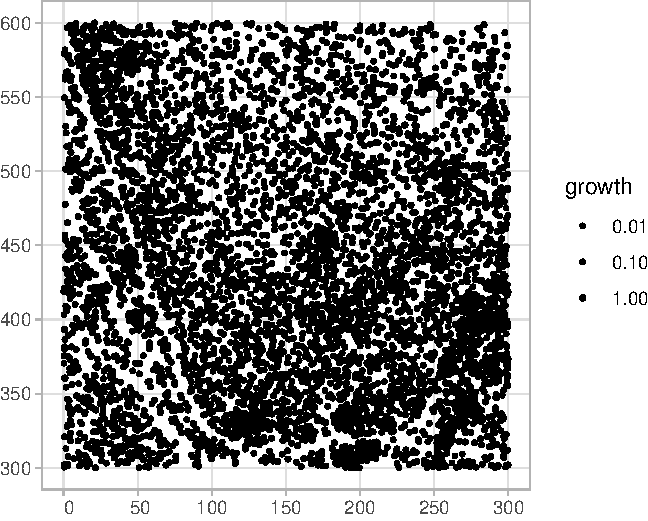
\includegraphics[width=0.66\linewidth]{Figures/scbi-trees-1} 

}

\caption{Step 1 - Compute growth of trees based on census data. A map of the growth of a random sample of 500 trees from a 9 ha subsection of the Smithsonian Conservation Biology Institute (SCBI) forest plot.}\label{fig:scbi-trees}
\end{figure}

\hypertarget{spatial-information}{%
\subsection{Step 2: Add spatial information}\label{spatial-information}}

We then add spatial information to \texttt{growth\_scbi}. We first add a
``buffer region'' to the periphery of the study region. Since some of
our model's explanatory variables are cumulative, we must ensure that
all trees being modeled are not biased to have different neighbor
structures. This is of concern for trees at the boundary of the study
region who will not have all their neighbors included in the census
stems. To account for such edge effects, only trees that are not part of
this buffer region, i.e.~are part of the interior of the study region,
will have their growth modeled \citep{waller_applied_2004}.

Our model of interspecific competition relies on a spatial definition of
who competitor trees are: all trees within a distance
\texttt{comp\_dist} of a focal tree. We set \texttt{comp\_dist} to 7.5m,
a value informed by other studies \citep[\citet{uriarte_spatially_2004},
\citet{canham_neighborhood_2006}]{canham_neighborhood_2004}. We use
\texttt{comp\_dist} and a manually constructed \texttt{sf}
representation of the study region's boundary as inputs to
\texttt{add\_buffer\_variable()} to add a \texttt{buffer} boolean
variable to \texttt{growth\_scbi}. All trees with \texttt{buffer} equal
to \texttt{FALSE} will be our focal trees whose growth will be modeled,
whereas those with \texttt{TRUE} will only act as competitor trees.

\begin{Shaded}
\begin{Highlighting}[]
\CommentTok{# Define competitive distance range}
\NormalTok{comp_dist <-}\StringTok{ }\FloatTok{7.5}

\CommentTok{# Manually construct study region boundary}
\NormalTok{study_region_scbi <-}\StringTok{ }\KeywordTok{tibble}\NormalTok{(}\DataTypeTok{x =} \KeywordTok{c}\NormalTok{(}\DecValTok{0}\NormalTok{, }\DecValTok{300}\NormalTok{, }\DecValTok{300}\NormalTok{, }\DecValTok{0}\NormalTok{, }\DecValTok{0}\NormalTok{), }\DataTypeTok{y =} \KeywordTok{c}\NormalTok{(}\DecValTok{300}\NormalTok{, }\DecValTok{300}\NormalTok{, }\DecValTok{600}\NormalTok{, }
    \DecValTok{600}\NormalTok{, }\DecValTok{300}\NormalTok{)) }\OperatorTok
\StringTok{    }\KeywordTok{sf_polygon}\NormalTok{()}

\NormalTok{growth_scbi <-}\StringTok{ }\NormalTok{growth_scbi }\OperatorTok
\StringTok{    }\KeywordTok{add_buffer_variable}\NormalTok{(}\DataTypeTok{size =}\NormalTok{ comp_dist, }\DataTypeTok{region =}\NormalTok{ study_region_scbi)}
\end{Highlighting}
\end{Shaded}

The second element of spatial information we add are blocks
corresponding to folds of a spatial cross-validation algorithm.
Conventional cross-validation algorithms assign individual observations
to folds by randomly resampling them all while assuming they are
statistically independent. In the case of forest census data however,
observations exhibit spatial autocorrelation. We therefore incorporate
this dependence into the cross-validation algorithm by resampling
spatial blocks of trees \citep[
\citet{pohjankukka_estimating_2017}]{roberts_cross-validation_2017}.

We first manually define an \texttt{sf} object defining four folds that
partition the study region. We then use the output of the
\texttt{spatialBlock()} function from the \texttt{blockCV} package to
associate each tree in \texttt{growth\_scbi} to the correct
\texttt{foldID} \citep{valavi_blockcv_2019}. This \texttt{foldID}
variable will be used in Section \ref{spatial-cross-validation}.

Figure \ref{fig:scbi-spatial-information} illustrates the net effect of
adding these two elements of spatial information to
\texttt{growth\_scbi}.

\begin{Shaded}
\begin{Highlighting}[]
\CommentTok{# Manually define spatial blocks to act as folds}
\NormalTok{n_fold <-}\StringTok{ }\DecValTok{4}
\NormalTok{fold1 <-}\StringTok{ }\KeywordTok{cbind}\NormalTok{(}\KeywordTok{c}\NormalTok{(}\DecValTok{0}\NormalTok{, }\DecValTok{150}\NormalTok{, }\DecValTok{150}\NormalTok{, }\DecValTok{0}\NormalTok{), }\KeywordTok{c}\NormalTok{(}\DecValTok{300}\NormalTok{, }\DecValTok{300}\NormalTok{, }\DecValTok{450}\NormalTok{, }\DecValTok{450}\NormalTok{))}
\NormalTok{fold2 <-}\StringTok{ }\KeywordTok{cbind}\NormalTok{(}\KeywordTok{c}\NormalTok{(}\DecValTok{150}\NormalTok{, }\DecValTok{300}\NormalTok{, }\DecValTok{300}\NormalTok{, }\DecValTok{150}\NormalTok{), }\KeywordTok{c}\NormalTok{(}\DecValTok{300}\NormalTok{, }\DecValTok{300}\NormalTok{, }\DecValTok{450}\NormalTok{, }\DecValTok{450}\NormalTok{))}
\NormalTok{fold3 <-}\StringTok{ }\KeywordTok{cbind}\NormalTok{(}\KeywordTok{c}\NormalTok{(}\DecValTok{0}\NormalTok{, }\DecValTok{150}\NormalTok{, }\DecValTok{150}\NormalTok{, }\DecValTok{0}\NormalTok{), }\KeywordTok{c}\NormalTok{(}\DecValTok{450}\NormalTok{, }\DecValTok{450}\NormalTok{, }\DecValTok{600}\NormalTok{, }\DecValTok{600}\NormalTok{))}
\NormalTok{fold4 <-}\StringTok{ }\KeywordTok{cbind}\NormalTok{(}\KeywordTok{c}\NormalTok{(}\DecValTok{150}\NormalTok{, }\DecValTok{300}\NormalTok{, }\DecValTok{300}\NormalTok{, }\DecValTok{150}\NormalTok{), }\KeywordTok{c}\NormalTok{(}\DecValTok{450}\NormalTok{, }\DecValTok{450}\NormalTok{, }\DecValTok{600}\NormalTok{, }\DecValTok{600}\NormalTok{))}

\NormalTok{blocks_scbi <-}\StringTok{ }\KeywordTok{bind_rows}\NormalTok{(}\KeywordTok{sf_polygon}\NormalTok{(fold1), }\KeywordTok{sf_polygon}\NormalTok{(fold2), }\KeywordTok{sf_polygon}\NormalTok{(fold3), }
    \KeywordTok{sf_polygon}\NormalTok{(fold4)) }\OperatorTok
\StringTok{    }\KeywordTok{mutate}\NormalTok{(}\DataTypeTok{folds =} \KeywordTok{c}\NormalTok{(}\DecValTok{1}\OperatorTok{:}\NormalTok{n_fold) }\OperatorTok
\StringTok{        }\KeywordTok{factor}\NormalTok{())}

\CommentTok{# Associate each observation to a fold}
\NormalTok{spatial_block_scbi <-}\StringTok{ }\KeywordTok{spatialBlock}\NormalTok{(}\DataTypeTok{speciesData =}\NormalTok{ growth_scbi, }\DataTypeTok{k =}\NormalTok{ n_fold, }
    \DataTypeTok{selection =} \StringTok{"systematic"}\NormalTok{, }\DataTypeTok{blocks =}\NormalTok{ blocks_scbi, }\DataTypeTok{showBlocks =} \OtherTok{FALSE}\NormalTok{, }\DataTypeTok{verbose =} \OtherTok{FALSE}\NormalTok{)}

\NormalTok{growth_scbi <-}\StringTok{ }\NormalTok{growth_scbi }\OperatorTok
\StringTok{    }\KeywordTok{mutate}\NormalTok{(}\DataTypeTok{foldID =}\NormalTok{ spatial_block_scbi}\OperatorTok{$}\NormalTok{foldID }\OperatorTok
\StringTok{        }\KeywordTok{factor}\NormalTok{())}
\end{Highlighting}
\end{Shaded}

\begin{Shaded}
\begin{Highlighting}[]
\KeywordTok{ggplot}\NormalTok{() }\OperatorTok{+}
\StringTok{  }\KeywordTok{geom_sf}\NormalTok{(}\DataTypeTok{data =}\NormalTok{ blocks_scbi, }\DataTypeTok{fill =} \StringTok{"transparent"}\NormalTok{, }\DataTypeTok{linetype =} \StringTok{"dashed"}\NormalTok{) }\OperatorTok{+}
\StringTok{  }\KeywordTok{geom_sf_text}\NormalTok{(}\DataTypeTok{data =}\NormalTok{ growth_scbi }\OperatorTok\StringTok{ }\KeywordTok{sample_n}\NormalTok{(}\DecValTok{1000}\NormalTok{), }
               \KeywordTok{aes}\NormalTok{(}\DataTypeTok{label =}\NormalTok{ foldID, }\DataTypeTok{col =}\NormalTok{ buffer))}
\end{Highlighting}
\end{Shaded}

\begin{figure}

{\centering 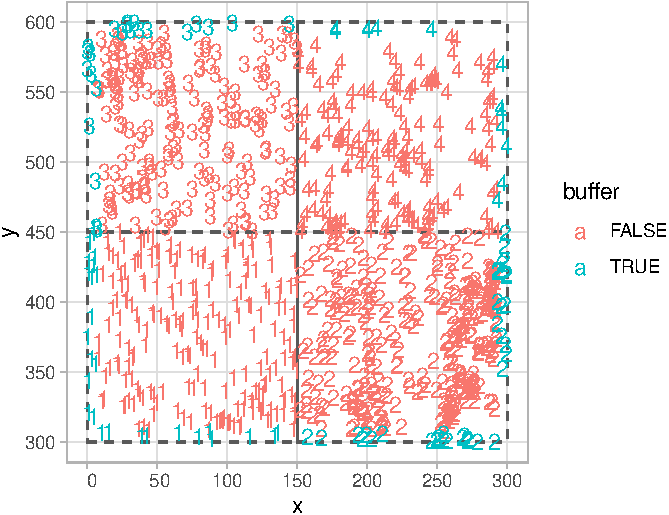
\includegraphics[width=0.66\linewidth]{Figures/scbi-spatial-information-1} 

}

\caption{Step 2 - Add spatial information. A buffer region and spatial cross-validation blocks 1 through 4. The location of each tree is marked with its fold number where the folds are delineated with solid lines. The color of each digit indicates whether the tree is part of the buffer region (thus will only be considered as a competitor tree) or is part of the interior of the study region (thus is a focal tree whose growth is of modeled interest).}\label{fig:scbi-spatial-information}
\end{figure}

\hypertarget{focal-vs-comp}{%
\subsection{Step 3: Identify all focal and corresponding competitor
trees}\label{focal-vs-comp}}

We then identify all focal trees and their corresponding competitor
trees. More specifically, identify all trees that are not part of the
buffer region, have a valid \texttt{growth} measurement, and have at
least one neighbor within 7.5m. We do this using
\texttt{create\_focal\_vs\_comp()}, which takes the previously detailed
\texttt{comp\_dist} and \texttt{id} arguments as well as the \texttt{sf}
representation of the spatial cross-validation blocks and returns a new
data frame \texttt{focal\_vs\_comp\_scbi}.

\begin{Shaded}
\begin{Highlighting}[]
\NormalTok{focal_vs_comp_scbi <-}\StringTok{ }\NormalTok{growth_scbi }\OperatorTok
\StringTok{  }\KeywordTok{create_focal_vs_comp}\NormalTok{(comp_dist, }\DataTypeTok{blocks =}\NormalTok{ blocks_scbi, }\DataTypeTok{id =} \StringTok{"stemID"}\NormalTok{)}
\NormalTok{focal_vs_comp_scbi }\OperatorTok\StringTok{ }
\StringTok{  }\KeywordTok{select}\NormalTok{(focal_ID, focal_sp, geometry, growth, comp)}
\CommentTok{## # A tibble: 6,296 x 5}
\CommentTok{##   focal_ID focal_sp   geometry growth comp             }
\CommentTok{##      <dbl> <fct>       <POINT>  <dbl> <list>           }
\CommentTok{## 1        4 nysy     (14.2 428)  0.103 <tibble [20 x 4]>}
\CommentTok{## 2        5 havi      (9.4 436)  0.150 <tibble [32 x 4]>}
\CommentTok{## 3       79 tiam       (40 381) -0.161 <tibble [20 x 4]>}
\CommentTok{## 4       80 caca     (38.7 422)  0.253 <tibble [12 x 4]>}
\CommentTok{## 5       96 libe       (60 310)  0.262 <tibble [14 x 4]>}
\CommentTok{## # ... with 6,291 more rows}
\end{Highlighting}
\end{Shaded}

The resulting \texttt{focal\_vs\_comp\_scbi} has 6296 rows, representing
the subset of the 7954 trees in \texttt{growth\_scbi} that will be
considered as focal trees. The variables \texttt{focal\_ID} and
\texttt{focal\_sp} relate to tree-stem identification and species
information. Most notably however is the variable \texttt{comp}, which
contains information on all competitor trees saved in \texttt{tidyr}
package list-column format \citep{tidyr_package}. To inspect this
information, we flatten the \texttt{comp} list-column for the tree with
\texttt{focal\_ID} 4 in the first row, here a
\texttt{tibble\ {[}20\ ×\ 4{]}}, into regular columns using
\texttt{unnest()} from the \texttt{tidyr} package.

\begin{Shaded}
\begin{Highlighting}[]
\NormalTok{focal_vs_comp_scbi }\OperatorTok
\StringTok{    }\KeywordTok{filter}\NormalTok{(focal_ID }\OperatorTok{==}\StringTok{ }\DecValTok{4}\NormalTok{) }\OperatorTok
\StringTok{    }\KeywordTok{select}\NormalTok{(focal_ID, dbh, comp) }\OperatorTok
\StringTok{    }\KeywordTok{unnest}\NormalTok{(}\DataTypeTok{cols =} \StringTok{"comp"}\NormalTok{)}
\CommentTok{## # A tibble: 20 x 6}
\CommentTok{##   focal_ID   dbh comp_ID  dist comp_sp comp_basal_area}
\CommentTok{##      <dbl> <dbl>   <dbl> <dbl> <fct>             <dbl>}
\CommentTok{## 1        4  13.6    1836  7.48 tiam            0.0176 }
\CommentTok{## 2        4  13.6    1847  2.81 nysy            0.00332}
\CommentTok{## 3        4  13.6    1848  1.62 nysy            0.00396}
\CommentTok{## 4        4  13.6    1849  2.62 nysy            0.00535}
\CommentTok{## 5        4  13.6    1850  2.98 havi            0.00472}
\CommentTok{## # ... with 15 more rows}
\end{Highlighting}
\end{Shaded}

We observe 4 variables describing 20 competitor trees: the unique
tree-stem ID, the distance to the focal tree (all \(\leq\) 7.5 m), the
species, and the basal area (in m\(^2\)) calculated as
\(\frac{\pi \times (\text{DBH/2})^2}{10000}\) for the DBH in cm from the
earlier census. Saving competitor information in list-column format
minimizes redundancy since we do not need to repeat information on the
focal tree 20 times. We visualize the spatial distribution of these
trees in Figure \ref{fig:scbi-focal-vs-comp-map}.

\begin{figure}

{\centering 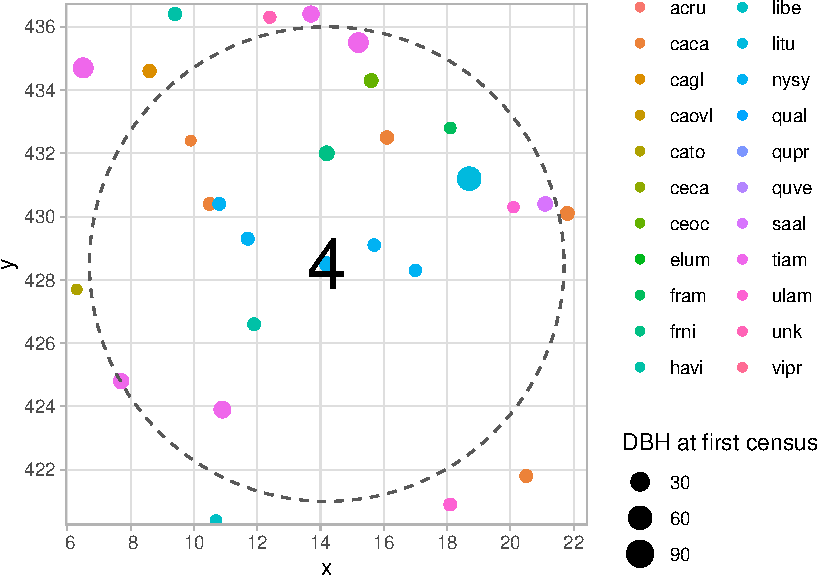
\includegraphics[width=0.66\linewidth]{Figures/scbi-focal-vs-comp-map-1} 

}

\caption{Step 3 - Identify all focal and corresponding competitor trees. The dashed circle extends 7.5m away from the focal tree 4 while all 20 competitor trees are within this circle.}\label{fig:scbi-focal-vs-comp-map}
\end{figure}

\hypertarget{model-fit-predict}{%
\subsection{Step 4: Fit model}\label{model-fit-predict}}

Lastly, we fit the competition Bayesian linear regression model for tree
growth outlined in Equation \ref{eq:model} using
\texttt{comp\_bayes\_lm()}. This function has an option to specify prior
distributions of all parameters, chosen here to be the defaults detailed
in \texttt{?comp\_bayes\_lm}.

\begin{Shaded}
\begin{Highlighting}[]
\NormalTok{comp_bayes_lm_scbi <-}\StringTok{ }\NormalTok{focal_vs_comp_scbi }\OperatorTok
\StringTok{  }\KeywordTok{comp_bayes_lm}\NormalTok{(}\DataTypeTok{prior_param =} \OtherTok{NULL}\NormalTok{)}
\end{Highlighting}
\end{Shaded}

The resulting\texttt{comp\_bayes\_lm\_scbi} is an object of S3 class
type \texttt{comp\_bayes\_lm} containing the posterior values of all
parameters. Furthermore, this class includes generics for three methods.
First, the generic for \texttt{print()} displays the names of all prior
and posterior parameters and the model formula:

\begin{Shaded}
\begin{Highlighting}[]
\NormalTok{comp_bayes_lm_scbi}
\CommentTok{## Bayesian linear regression model parameters with a multivariate Normal}
\CommentTok{## likelihood. See ?comp_bayes_lm for details:}
\CommentTok{## }
\CommentTok{##   parameter_type           prior posterior}
\CommentTok{## 1 Inverse-Gamma on sigma^2 a_0   a_star   }
\CommentTok{## 2 Inverse-Gamma on sigma^2 b_0   b_star   }
\CommentTok{## 3 Multivariate t on beta   mu_0  mu_star  }
\CommentTok{## 4 Multivariate t on beta   V_0   V_star   }
\CommentTok{## }
\CommentTok{## Model formula:}
\CommentTok{## growth ~ sp + dbh + dbh * sp + acne * sp + acru * sp + amar * sp + astr}
\CommentTok{## * sp + caca * sp + caco * sp + cade * sp + cagl * sp + caovl * sp + cato}
\CommentTok{## * sp + ceca * sp + ceoc * sp + chvi * sp + cofl * sp + crpr * sp + crsp}
\CommentTok{## * sp + divi * sp + elum * sp + fagr * sp + fram * sp + frni * sp + frpe}
\CommentTok{## * sp + havi * sp + ilve * sp + juci * sp + juni * sp + libe * sp + litu}
\CommentTok{## * sp + nysy * sp + pist * sp + pivi * sp + ploc * sp + prav * sp + prse}
\CommentTok{## * sp + qual * sp + quco * sp + qufa * sp + qumi * sp + qupr * sp + quru}
\CommentTok{## * sp + quve * sp + rops * sp + saal * sp + saca * sp + tiam * sp + ulam}
\CommentTok{## * sp + ulru * sp + unk * sp + vipr * sp}
\end{Highlighting}
\end{Shaded}

Next, the generic for \texttt{predict()} takes the posterior parameter
values in \texttt{comp\_bayes\_lm\_scbi} and a \texttt{newdata} data
frame, and outputs a vector \texttt{growth\_hat} of predicted DBH values
\(\widehat{y_{ij}}\) computed from the posterior predictive
distribution.

\begin{Shaded}
\begin{Highlighting}[]
\NormalTok{focal_vs_comp_scbi <-}\StringTok{ }\NormalTok{focal_vs_comp_scbi }\OperatorTok
\StringTok{  }\KeywordTok{mutate}\NormalTok{(}\DataTypeTok{growth_hat =} \KeywordTok{predict}\NormalTok{(comp_bayes_lm_scbi, }\DataTypeTok{newdata =}\NormalTok{ focal_vs_comp_scbi))}
\end{Highlighting}
\end{Shaded}

\begin{Shaded}
\begin{Highlighting}[]
\NormalTok{focal_vs_comp_scbi }\OperatorTok
\StringTok{    }\KeywordTok{select}\NormalTok{(focal_ID, focal_sp, dbh, growth, growth_hat)}
\CommentTok{## # A tibble: 6,296 x 5}
\CommentTok{##   focal_ID focal_sp   dbh growth growth_hat}
\CommentTok{##      <dbl> <fct>    <dbl>  <dbl>      <dbl>}
\CommentTok{## 1        4 nysy     13.6   0.103     0.0809}
\CommentTok{## 2        5 havi      8.8   0.150     0.112 }
\CommentTok{## 3       79 tiam     47.7  -0.161     0.229 }
\CommentTok{## 4       80 caca      5.15  0.253     0.121 }
\CommentTok{## 5       96 libe      2.3   0.262     0.142 }
\CommentTok{## # ... with 6,291 more rows}
\end{Highlighting}
\end{Shaded}

We can now compare the observed and predicted growths to compute the
root mean squared error (RMSE) of our model:

\begin{Shaded}
\begin{Highlighting}[]
\NormalTok{model_rmse <-}\StringTok{ }\NormalTok{focal_vs_comp_scbi }\OperatorTok
\StringTok{  }\KeywordTok{rmse}\NormalTok{(}\DataTypeTok{truth =}\NormalTok{ growth, }\DataTypeTok{estimate =}\NormalTok{ growth_hat) }\OperatorTok
\StringTok{  }\KeywordTok{pull}\NormalTok{(.estimate)}
\NormalTok{model_rmse}
\CommentTok{## [1] 0.128}
\end{Highlighting}
\end{Shaded}

Lastly, the generic for \texttt{ggplot2::autoplot()} allows us to
visualize all posterior distributions, as seen in Figure
\ref{fig:scbi-posterior-viz}. Setting \texttt{type} to
\texttt{"intercepts"} and \texttt{"dbh\_slopes"} returns
species-specific posterior distributions for \(\beta_{0,j}\) and
\(\beta_{dbh,j}\) respectively, while setting
\texttt{type\ =\ "competition"} returns competition coefficients
\(\lambda_{j,k}\).

\begin{Shaded}
\begin{Highlighting}[]
\CommentTok{# Plot posteriors for only a subset of species}
\NormalTok{sp_to_plot <-}\StringTok{ }\KeywordTok{c}\NormalTok{(}\StringTok{"litu"}\NormalTok{, }\StringTok{"quru"}\NormalTok{, }\StringTok{"cagl"}\NormalTok{)}

\NormalTok{plot1 <-}\StringTok{ }\KeywordTok{autoplot}\NormalTok{(comp_bayes_lm_scbi, }\DataTypeTok{type =} \StringTok{"intercepts"}\NormalTok{, }
                  \DataTypeTok{sp_to_plot =}\NormalTok{ sp_to_plot)}
\NormalTok{plot2 <-}\StringTok{ }\KeywordTok{autoplot}\NormalTok{(comp_bayes_lm_scbi, }\DataTypeTok{type =} \StringTok{"dbh_slopes"}\NormalTok{, }
                  \DataTypeTok{sp_to_plot =}\NormalTok{ sp_to_plot)}
\NormalTok{plot3 <-}\StringTok{ }\KeywordTok{autoplot}\NormalTok{(comp_bayes_lm_scbi, }\DataTypeTok{type =} \StringTok{"competition"}\NormalTok{, }
                  \DataTypeTok{sp_to_plot =}\NormalTok{ sp_to_plot)}

\CommentTok{# Combine plots using the patchwork package}
\NormalTok{(plot1 }\OperatorTok{|}\StringTok{ }\NormalTok{plot2) }\OperatorTok{/}\StringTok{ }\NormalTok{plot3}
\end{Highlighting}
\end{Shaded}

\begin{figure}

{\centering 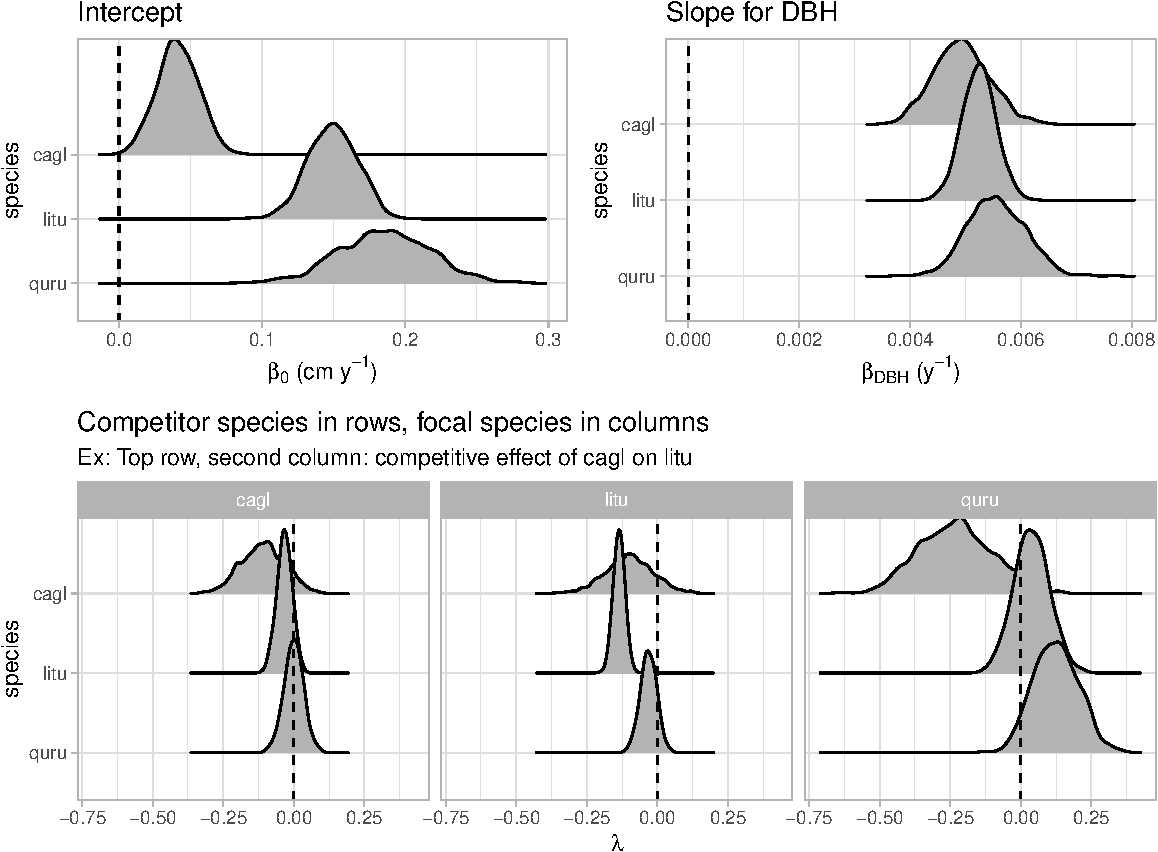
\includegraphics[width=1\linewidth]{Figures/scbi-posterior-viz-1} 

}

\caption{Step 4 - Fit model. Posterior distributions of all parameters. For compactness we include only three species.}\label{fig:scbi-posterior-viz}
\end{figure}

For many users the visualizations of \(\lambda_{j,k}\) will be of
particular interest as they provide insight into species-specific
competitive interactions, where negative values indicate a competitor
species which slows the growth of a focal species. Here, for example, we
see that tulip poplars (litu) have a strong negative effect on the
growth of conspecifics but relatively lesser effect on pignut hickory
(cagl) and red oak (quru) neighbors.

Currently the \texttt{forestecology} package can only fit the
competition Bayesian linear regression model in Equation \ref{eq:model}.
However, it can be extended to any model as long as it is implemented in
a function similar to \texttt{comp\_bayes\_lm()}.

\hypertarget{permutation-test}{%
\subsection{Evaluate the effect of competitor species identity using
permutation tests}\label{permutation-test}}

To evaluate the effect of competitor species identity, we use the above
four steps along with the permutation test in Equation
\ref{eq:permutation-hypothesis-test}. Under a null hypothesis where
competitor species identity does not matter, we can permute the
competitor species identities within each focal tree, compute the RMSE
test statistic, repeat this process several times to construct a null
distribution, and compare it to the observed RMSE to assess
significance. Going back to our example in Section \ref{focal-vs-comp}
of focal tree with \texttt{focal\_ID} 4 and its 20 competitors, the
permutation test only randomly resamples the \texttt{comp\_sp} variable
without replacement, leaving all other variables intact. This resampling
is nested within each focal tree in order to preserve neighborhood
structure. We perform this permutation test once again using
\texttt{comp\_bayes\_lm()} but by setting
\texttt{run\_shuffle\ =\ TRUE}.

\begin{Shaded}
\begin{Highlighting}[]
\NormalTok{comp_bayes_lm_scbi_shuffle <-}\StringTok{ }\NormalTok{focal_vs_comp_scbi }\OperatorTok
\StringTok{  }\KeywordTok{comp_bayes_lm}\NormalTok{(}\DataTypeTok{prior_param =} \OtherTok{NULL}\NormalTok{, }\DataTypeTok{run_shuffle =} \OtherTok{TRUE}\NormalTok{)}

\NormalTok{focal_vs_comp_scbi <-}\StringTok{ }\NormalTok{focal_vs_comp_scbi }\OperatorTok
\StringTok{  }\KeywordTok{mutate}\NormalTok{(}\DataTypeTok{growth_hat_shuffle =} \KeywordTok{predict}\NormalTok{(comp_bayes_lm_scbi_shuffle, }
                                 \DataTypeTok{newdata =}\NormalTok{ focal_vs_comp_scbi))}
\end{Highlighting}
\end{Shaded}

\begin{Shaded}
\begin{Highlighting}[]
\NormalTok{model_rmse_shuffle <-}\StringTok{ }\NormalTok{focal_vs_comp_scbi }\OperatorTok
\StringTok{    }\KeywordTok{rmse}\NormalTok{(}\DataTypeTok{truth =}\NormalTok{ growth, }\DataTypeTok{estimate =}\NormalTok{ growth_hat_shuffle) }\OperatorTok
\StringTok{    }\KeywordTok{pull}\NormalTok{(.estimate)}
\NormalTok{model_rmse_shuffle}
\CommentTok{## [1] 0.131}
\end{Highlighting}
\end{Shaded}

The resulting permutation test RMSE of 0.131 is larger than the earlier
RMSE of 0.128, suggesting that models that do incorporate competitor
species identity better fit the data.

\hypertarget{spatial-cross-validation}{%
\subsection{Evaluate model performance using spatial
cross-validation}\label{spatial-cross-validation}}

To evaluate model performance, we use spatial cross-validation. The
model fit in Section \ref{model-fit-predict} uses the same data to both
fit and assess model performance. Given the spatial-autocorrelation of
our data, this can potentially lead to overfit models
\citep{roberts_cross-validation_2017}. To mitigate this risk, we use the
spatial cross-validation blocking scheme encoded in the \texttt{foldID}
variable from Section \ref{spatial-information} and visualized in Figure
\ref{fig:scbi-spatial-information}.

At each iteration of the cross-validation, one fold acts as the test set
and the remaining three act as the training set. We fit the model to all
focal trees in the training set, apply the model to all focal trees in
the test set, compute predicted values, and compute the RMSE.
Furthermore, to maintain spatial independence between the test and
training sets, a ``fold buffer'' that extends 7.5m outwards from the
boundary of the test set is considered; all trees within this ``fold
buffer'' are excluded from the training set (see Figure
\ref{fig:scbi-spatial-cross-validation-schematic}).

\begin{figure}

{\centering 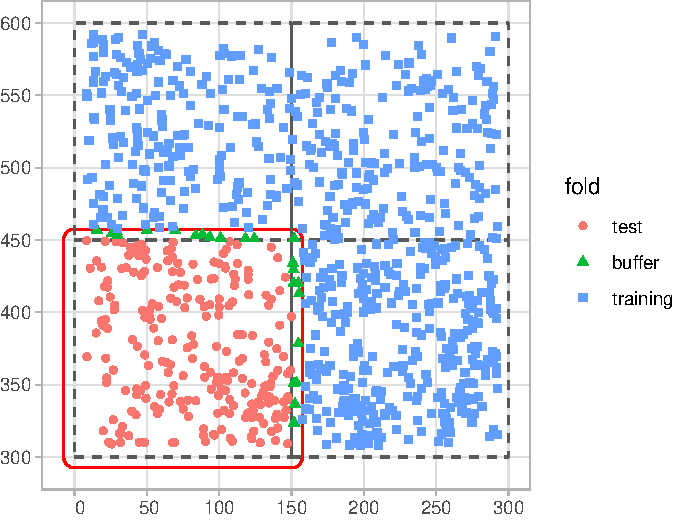
\includegraphics[width=0.66\linewidth]{Figures/scbi-spatial-cross-validation-schematic-1} 

}

\caption{Schematic of spatial cross-validation. Using the k = 1 fold (bottom-left) as the test set, k = 2 through 4 as the training set, along with a "fold buffer" extending outwards from the test set to maintain spatial independence between it and the training set.}\label{fig:scbi-spatial-cross-validation-schematic}
\end{figure}

This process is repeated for each of the four folds acting as the test
set, then the four RMSE's are averaged to provide a single estimate of
model error. This algorithm is implemented in \texttt{run\_cv()}, which
acts as a wrapper function to both \texttt{comp\_bayes\_lm()} that fits
the model and \texttt{predict()} that returns predicted values.

\begin{Shaded}
\begin{Highlighting}[]
\NormalTok{focal_vs_comp_scbi <-}\StringTok{ }\NormalTok{focal_vs_comp_scbi }\OperatorTok
\StringTok{  }\KeywordTok{run_cv}\NormalTok{(}\DataTypeTok{comp_dist =}\NormalTok{ comp_dist, }\DataTypeTok{blocks =}\NormalTok{ blocks_scbi)}
\end{Highlighting}
\end{Shaded}

\begin{Shaded}
\begin{Highlighting}[]
\NormalTok{model_rmse_cv <-}\StringTok{ }\NormalTok{focal_vs_comp_scbi }\OperatorTok
\StringTok{    }\KeywordTok{rmse}\NormalTok{(}\DataTypeTok{truth =}\NormalTok{ growth, }\DataTypeTok{estimate =}\NormalTok{ growth_hat) }\OperatorTok
\StringTok{    }\KeywordTok{pull}\NormalTok{(.estimate)}
\NormalTok{model_rmse_cv}
\CommentTok{## [1] 0.14}
\end{Highlighting}
\end{Shaded}

The resulting RMSE of 0.14 computed using cross-validation is larger
than the earlier RMSE of 0.128, suggesting that models that do not
account for spatial autocorrelation generate model error estimates that
are overly optimistic, i.e.~RMSE values that are too low.

\hypertarget{importance-of-spatial-cross-validation}{%
\section{Importance of spatial
cross-validation}\label{importance-of-spatial-cross-validation}}

\texttt{run\_cv()} also accepts the \texttt{run\_shuffle} argument in
order to permute competitor species identity as described in Section
\ref{permutation-test}. Figure \ref{fig:scbi-simulation} compares model
performance for 49 permutations of competitor species and RMSE
calculations, both with and without cross-validation. Without
cross-validation, competitor species identity does matter as the
observed RMSE was significantly lower than the permutation null
distribution of RMSE. However, once we incorporate spatial
cross-validation, this improvement disappears. These results suggest
that in this 9 ha subplot of the SCBI plot, competitive interactions do
not depend on the identity of the competitor, which is the opposite of
what has been observed in other locations \citep[
\citet{uriarte_spatially_2004}]{allen_permutation_2020}. This provides a
striking example of the importance of cross-validation, as without it
the over-fit model gives rise to an incorrect conclusion.

\begin{figure}

{\centering 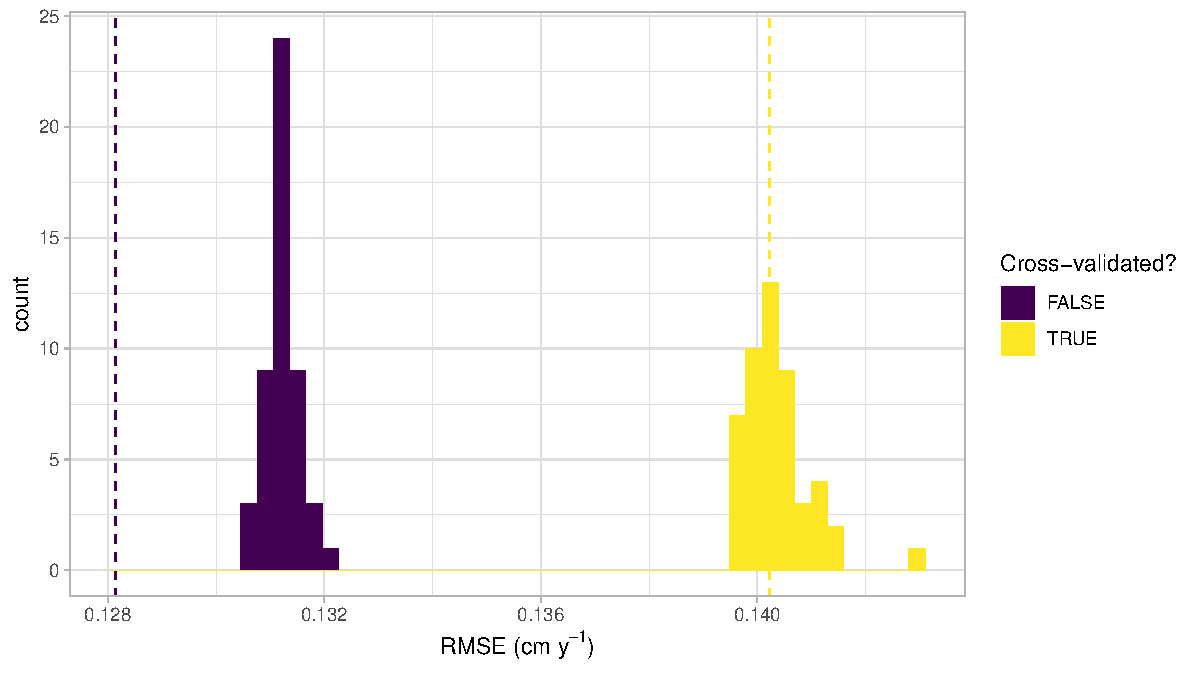
\includegraphics[width=1\linewidth]{simulation_results/2021-03-03_scbi_49_shuffles} 

}

\caption{Comparison of root mean squared error of models for standard, permuted, and spatially cross-validated error estimates. The dotted lines show observed RMSE while the histograms show the null distribution of RMSE for 49 permutations under the null hypothesis of no competitor species identity effects. The colors indicate whether spatial cross-validation was used or not.}\label{fig:scbi-simulation}
\end{figure}

\hypertarget{conclusion-and-future-work}{%
\section{Conclusion and future work}\label{conclusion-and-future-work}}

The \texttt{forestecology} package provides an accessible way to fit and
test models of neighborhood competition. The package follows the
\texttt{tidy} data design principles, leverages the \texttt{sf} package
for spatial data, and S3 open-oriented model implementation structure.
We hope that the package will increase the use of neighborhood
competition models to better understand what structures plant
competition.

While the package is designed with ForestGEO plot data in mind, we
envision that it can be modified to work on any single large, mapped
forest plot in which at least two measurements of each individual have
been taken. Furthermore, we hope that future versions of the package
will be flexible to other plot layouts, for example inventory
plot-structure with many spatially separated plots like the US Forest
Service Forest Inventory and Analysis plots \citep{smith_forest_2002}.

We also hope to extend the \texttt{forestecology} package's
functionality to account for a larger variety of models for tree growth.
One clear future direction would be to allow competition based on
species trait values rather than species identity. There is evidence
that traits predict competitive outcomes
\citep[\citet{lasky_trait-mediated_2014},
\citet{uriarte_trait_2010}]{kunstler_competitive_2012}. Thus an
extension of the model would allow \(\lambda\) values from Equation
\ref{eq:model} to be a function of the traits of competing species.

Lastly, the \texttt{forestecology} current uses the \texttt{blockCV}
package behind the scenes to create the spatial blocks acting as folds
for our spatial cross-validation algorithm detailed in Sections
\ref{spatial-information} and \ref{spatial-cross-validation}
\citep{valavi_blockcv_2019}. This back-end functionality could be
substituted with the \texttt{spatialsample} package for spatial
resampling infrastructure; a \texttt{tidymodels} package under active
development as of 2021
\citep[\citet{tidymodels_package}]{spatialsample_package}.

\hypertarget{acknowledgments}{%
\section{Acknowledgments}\label{acknowledgments}}

We thank Sophie Li for their feedback on the package interface. The
authors declare no conflicts of interest.

\hypertarget{authors-contributions}{%
\section{Author's contributions}\label{authors-contributions}}

AYK and DNA conceived the ideas and coded a draft of the package. AYK
wrote an initial manuscript draft. SPC rewrote much of the package's
code to align with R and ``tidy'' best practices
\citep{wickham_welcome_2019}. All authors contributed to subsequent
drafts and gave final approval for manuscript.

\hypertarget{data-accessibility}{%
\section{Data accessibility}\label{data-accessibility}}

We intend to archive all data and source code for this manuscript on
GitHub at \url{https://github.com/rudeboybert/forestecology} and on
Zenodo upon acceptance. The example Smithsonian Conservation Biology
Institute census data are available on GitHub at
\url{https://github.com/SCBI-ForestGEO/SCBI-ForestGEO-Data/tree/master/tree_main_census/data/census-csv-files}
and are archived on Zenodo at
\url{https://doi.org/10.5281/zenodo.2649301}
\citep{gonzalez-akre_scbi-forestgeoscbi-forestgeo-data_2020}.

\hypertarget{appendix}{%
\section{Appendix}\label{appendix}}

This code replicates Figure \ref{fig:scbi-simulation}: A comparison of
root mean squared error of models for standard, permuted, and spatial
cross- validated error estimates.

\begin{Shaded}
\begin{Highlighting}[]
\KeywordTok{library}\NormalTok{(tidyverse)}
\KeywordTok{library}\NormalTok{(lubridate)}
\KeywordTok{library}\NormalTok{(here)}
\KeywordTok{library}\NormalTok{(sf)}
\KeywordTok{library}\NormalTok{(viridis)}
\KeywordTok{library}\NormalTok{(forestecology)}
\KeywordTok{library}\NormalTok{(blockCV)}
\KeywordTok{library}\NormalTok{(tictoc)}


\CommentTok{# Compute growth of trees based on census data -------------------------}
\NormalTok{census_}\DecValTok{2013}\NormalTok{_scbi <-}\StringTok{ }\KeywordTok{here}\NormalTok{(}\StringTok{"paper/scbi.stem2.csv"}\NormalTok{) }\OperatorTok
\StringTok{    }\KeywordTok{read_csv}\NormalTok{() }\OperatorTok
\StringTok{    }\KeywordTok{select}\NormalTok{(stemID, sp, }\DataTypeTok{date =}\NormalTok{ ExactDate, gx, gy, dbh, codes, status) }\OperatorTok
\StringTok{    }\KeywordTok{mutate}\NormalTok{(}\DataTypeTok{date =} \KeywordTok{mdy}\NormalTok{(date), }\DataTypeTok{dbh =} \KeywordTok{as.numeric}\NormalTok{(dbh)}\OperatorTok{/}\DecValTok{10}\NormalTok{) }\OperatorTok
\StringTok{    }\KeywordTok{filter}\NormalTok{(gx }\OperatorTok{<}\StringTok{ }\DecValTok{300}\NormalTok{, }\KeywordTok{between}\NormalTok{(gy, }\DecValTok{300}\NormalTok{, }\DecValTok{600}\NormalTok{))}

\NormalTok{census_}\DecValTok{2018}\NormalTok{_scbi <-}\StringTok{ }\KeywordTok{here}\NormalTok{(}\StringTok{"paper/scbi.stem3.csv"}\NormalTok{) }\OperatorTok
\StringTok{    }\KeywordTok{read_csv}\NormalTok{() }\OperatorTok
\StringTok{    }\KeywordTok{select}\NormalTok{(stemID, sp, }\DataTypeTok{date =}\NormalTok{ ExactDate, gx, gy, dbh, codes, status) }\OperatorTok
\StringTok{    }\KeywordTok{mutate}\NormalTok{(}\DataTypeTok{date =} \KeywordTok{mdy}\NormalTok{(date), }\DataTypeTok{dbh =} \KeywordTok{as.numeric}\NormalTok{(dbh)}\OperatorTok{/}\DecValTok{10}\NormalTok{) }\OperatorTok
\StringTok{    }\KeywordTok{filter}\NormalTok{(gx }\OperatorTok{<}\StringTok{ }\DecValTok{300}\NormalTok{, }\KeywordTok{between}\NormalTok{(gy, }\DecValTok{300}\NormalTok{, }\DecValTok{600}\NormalTok{))}

\NormalTok{growth_scbi <-}\StringTok{ }\KeywordTok{compute_growth}\NormalTok{(}\DataTypeTok{census_1 =}\NormalTok{ census_}\DecValTok{2013}\NormalTok{_scbi, }\DataTypeTok{census_2 =}\NormalTok{ census_}\DecValTok{2018}\NormalTok{_scbi }\OperatorTok
\StringTok{    }\KeywordTok{filter}\NormalTok{(}\OperatorTok{!}\KeywordTok{str_detect}\NormalTok{(codes, }\StringTok{"R"}\NormalTok{)), }\DataTypeTok{id =} \StringTok{"stemID"}\NormalTok{)}


\CommentTok{# Add spatial information ----------------------------------------------}
\CommentTok{# Define buffer region using competitive distance range}
\NormalTok{comp_dist <-}\StringTok{ }\FloatTok{7.5}

\NormalTok{study_region_scbi <-}\StringTok{ }\KeywordTok{tibble}\NormalTok{(}\DataTypeTok{x =} \KeywordTok{c}\NormalTok{(}\DecValTok{0}\NormalTok{, }\DecValTok{300}\NormalTok{, }\DecValTok{300}\NormalTok{, }\DecValTok{0}\NormalTok{, }\DecValTok{0}\NormalTok{), }\DataTypeTok{y =} \KeywordTok{c}\NormalTok{(}\DecValTok{300}\NormalTok{, }\DecValTok{300}\NormalTok{, }\DecValTok{600}\NormalTok{, }
    \DecValTok{600}\NormalTok{, }\DecValTok{300}\NormalTok{)) }\OperatorTok
\StringTok{    }\KeywordTok{sf_polygon}\NormalTok{()}

\NormalTok{growth_scbi <-}\StringTok{ }\NormalTok{growth_scbi }\OperatorTok
\StringTok{    }\KeywordTok{add_buffer_variable}\NormalTok{(}\DataTypeTok{size =}\NormalTok{ comp_dist, }\DataTypeTok{region =}\NormalTok{ study_region_scbi)}

\CommentTok{# Manually define spatial blocks to act as folds}
\NormalTok{fold1 <-}\StringTok{ }\KeywordTok{rbind}\NormalTok{(}\KeywordTok{c}\NormalTok{(}\DecValTok{0}\NormalTok{, }\DecValTok{300}\NormalTok{), }\KeywordTok{c}\NormalTok{(}\DecValTok{150}\NormalTok{, }\DecValTok{300}\NormalTok{), }\KeywordTok{c}\NormalTok{(}\DecValTok{150}\NormalTok{, }\DecValTok{450}\NormalTok{), }\KeywordTok{c}\NormalTok{(}\DecValTok{0}\NormalTok{, }\DecValTok{450}\NormalTok{))}
\NormalTok{fold2 <-}\StringTok{ }\KeywordTok{rbind}\NormalTok{(}\KeywordTok{c}\NormalTok{(}\DecValTok{150}\NormalTok{, }\DecValTok{300}\NormalTok{), }\KeywordTok{c}\NormalTok{(}\DecValTok{300}\NormalTok{, }\DecValTok{300}\NormalTok{), }\KeywordTok{c}\NormalTok{(}\DecValTok{300}\NormalTok{, }\DecValTok{450}\NormalTok{), }\KeywordTok{c}\NormalTok{(}\DecValTok{150}\NormalTok{, }\DecValTok{450}\NormalTok{))}
\NormalTok{fold3 <-}\StringTok{ }\KeywordTok{rbind}\NormalTok{(}\KeywordTok{c}\NormalTok{(}\DecValTok{0}\NormalTok{, }\DecValTok{450}\NormalTok{), }\KeywordTok{c}\NormalTok{(}\DecValTok{150}\NormalTok{, }\DecValTok{450}\NormalTok{), }\KeywordTok{c}\NormalTok{(}\DecValTok{150}\NormalTok{, }\DecValTok{600}\NormalTok{), }\KeywordTok{c}\NormalTok{(}\DecValTok{0}\NormalTok{, }\DecValTok{600}\NormalTok{))}
\NormalTok{fold4 <-}\StringTok{ }\KeywordTok{rbind}\NormalTok{(}\KeywordTok{c}\NormalTok{(}\DecValTok{150}\NormalTok{, }\DecValTok{450}\NormalTok{), }\KeywordTok{c}\NormalTok{(}\DecValTok{300}\NormalTok{, }\DecValTok{450}\NormalTok{), }\KeywordTok{c}\NormalTok{(}\DecValTok{300}\NormalTok{, }\DecValTok{600}\NormalTok{), }\KeywordTok{c}\NormalTok{(}\DecValTok{150}\NormalTok{, }\DecValTok{600}\NormalTok{))}
\NormalTok{n_fold <-}\StringTok{ }\DecValTok{4}

\NormalTok{blocks_scbi <-}\StringTok{ }\KeywordTok{bind_rows}\NormalTok{(}\KeywordTok{sf_polygon}\NormalTok{(fold1), }\KeywordTok{sf_polygon}\NormalTok{(fold2), }\KeywordTok{sf_polygon}\NormalTok{(fold3), }
    \KeywordTok{sf_polygon}\NormalTok{(fold4)) }\OperatorTok
\StringTok{    }\KeywordTok{mutate}\NormalTok{(}\DataTypeTok{folds =} \KeywordTok{c}\NormalTok{(}\DecValTok{1}\OperatorTok{:}\NormalTok{n_fold) }\OperatorTok
\StringTok{        }\KeywordTok{factor}\NormalTok{())}

\CommentTok{# Associate each observation to a fold}
\NormalTok{SpatialBlock_scbi <-}\StringTok{ }\KeywordTok{spatialBlock}\NormalTok{(}\DataTypeTok{speciesData =}\NormalTok{ growth_scbi, }\DataTypeTok{k =}\NormalTok{ n_fold, }
    \DataTypeTok{selection =} \StringTok{"systematic"}\NormalTok{, }\DataTypeTok{blocks =}\NormalTok{ blocks_scbi, }\DataTypeTok{showBlocks =} \OtherTok{FALSE}\NormalTok{, }\DataTypeTok{verbose =} \OtherTok{FALSE}\NormalTok{)}

\NormalTok{growth_scbi <-}\StringTok{ }\NormalTok{growth_scbi }\OperatorTok
\StringTok{    }\KeywordTok{mutate}\NormalTok{(}\DataTypeTok{foldID =}\NormalTok{ SpatialBlock_scbi}\OperatorTok{$}\NormalTok{foldID }\OperatorTok
\StringTok{        }\KeywordTok{factor}\NormalTok{())}


\CommentTok{# Compute focal versus competitor tree information ---------------------}
\NormalTok{focal_vs_comp_scbi <-}\StringTok{ }\NormalTok{growth_scbi }\OperatorTok
\StringTok{    }\KeywordTok{create_focal_vs_comp}\NormalTok{(comp_dist, }\DataTypeTok{blocks =}\NormalTok{ blocks_scbi, }\DataTypeTok{id =} \StringTok{"stemID"}\NormalTok{)}


\CommentTok{# Fit model and make predictions ---------------------------------------}
\CommentTok{# Number of permutation shuffles:}
\NormalTok{num_shuffle <-}\StringTok{ }\DecValTok{49}

\CommentTok{# Save results here}
\NormalTok{run_time <-}\StringTok{ }\DecValTok{0}
\NormalTok{observed_RMSE <-}\StringTok{ }\DecValTok{0}
\NormalTok{observed_RMSE_CV <-}\StringTok{ }\DecValTok{0}
\NormalTok{shuffle_RMSE <-}\StringTok{ }\KeywordTok{vector}\NormalTok{(}\StringTok{"list"}\NormalTok{, }\DecValTok{1}\NormalTok{)}
\NormalTok{shuffle_RMSE_CV <-}\StringTok{ }\KeywordTok{vector}\NormalTok{(}\StringTok{"list"}\NormalTok{, }\DecValTok{1}\NormalTok{)}
\NormalTok{filename <-}\StringTok{ }\KeywordTok{here}\NormalTok{(}\StringTok{"paper/simulation_results/"}\NormalTok{) }\OperatorTok
\StringTok{    }\KeywordTok{str_c}\NormalTok{(}\StringTok{"2021-03-03_scbi_"}\NormalTok{, num_shuffle, }\StringTok{"_shuffles"}\NormalTok{)}

\CommentTok{# Run all simulations 0. Setup simulation for this species type ----}
\CommentTok{# Start clock}
\KeywordTok{tic}\NormalTok{()}

\CommentTok{# 1. Compute observed test statistic: RMSE with no cross-validation ----}
\CommentTok{# Fit model (compute posterior parameters)}
\NormalTok{comp_bayes_lm_scbi <-}\StringTok{ }\NormalTok{focal_vs_comp_scbi }\OperatorTok
\StringTok{    }\KeywordTok{comp_bayes_lm}\NormalTok{(}\DataTypeTok{prior_param =} \OtherTok{NULL}\NormalTok{, }\DataTypeTok{run_shuffle =} \OtherTok{FALSE}\NormalTok{)}

\CommentTok{# Make predictions and compute RMSE}
\NormalTok{observed_RMSE <-}\StringTok{ }\NormalTok{focal_vs_comp_scbi }\OperatorTok
\StringTok{    }\KeywordTok{mutate}\NormalTok{(}\DataTypeTok{growth_hat =} \KeywordTok{predict}\NormalTok{(comp_bayes_lm_scbi, focal_vs_comp_scbi)) }\OperatorTok
\StringTok{    }\KeywordTok{rmse}\NormalTok{(}\DataTypeTok{truth =}\NormalTok{ growth, }\DataTypeTok{estimate =}\NormalTok{ growth_hat) }\OperatorTok
\StringTok{    }\KeywordTok{pull}\NormalTok{(.estimate)}

\CommentTok{# 2. Compute observed test statistic: RMSE with cross-validation -------}
\NormalTok{observed_RMSE_CV <-}\StringTok{ }\NormalTok{focal_vs_comp_scbi }\OperatorTok
\StringTok{    }\KeywordTok{run_cv}\NormalTok{(}\DataTypeTok{comp_dist =}\NormalTok{ comp_dist, }\DataTypeTok{blocks =}\NormalTok{ blocks_scbi) }\OperatorTok
\StringTok{    }\KeywordTok{rmse}\NormalTok{(}\DataTypeTok{truth =}\NormalTok{ growth, }\DataTypeTok{estimate =}\NormalTok{ growth_hat) }\OperatorTok
\StringTok{    }\KeywordTok{pull}\NormalTok{(.estimate)}

\CommentTok{# 3. Permutation distribution: RMSE with no cross-validation -----------}
\CommentTok{# Compute num_shuffle permutation test statistics}
\NormalTok{shuffle_RMSE <-}\StringTok{ }\KeywordTok{numeric}\NormalTok{(}\DataTypeTok{length =}\NormalTok{ num_shuffle)}
\ControlFlowTok{for}\NormalTok{ (j }\ControlFlowTok{in} \DecValTok{1}\OperatorTok{:}\NormalTok{num_shuffle) \{}
    \CommentTok{# Fit model (compute posterior parameters) with shuffling}
\NormalTok{    comp_bayes_lm_scbi <-}\StringTok{ }\NormalTok{focal_vs_comp_scbi }\OperatorTok
\StringTok{        }\KeywordTok{comp_bayes_lm}\NormalTok{(}\DataTypeTok{prior_param =} \OtherTok{NULL}\NormalTok{, }\DataTypeTok{run_shuffle =} \OtherTok{TRUE}\NormalTok{)}

    \CommentTok{# Make predictions and compute RMSE}
\NormalTok{    shuffle_RMSE[j] <-}\StringTok{ }\NormalTok{focal_vs_comp_scbi }\OperatorTok
\StringTok{        }\KeywordTok{mutate}\NormalTok{(}\DataTypeTok{growth_hat =} \KeywordTok{predict}\NormalTok{(comp_bayes_lm_scbi, focal_vs_comp_scbi)) }\OperatorTok
\StringTok{        }\KeywordTok{rmse}\NormalTok{(}\DataTypeTok{truth =}\NormalTok{ growth, }\DataTypeTok{estimate =}\NormalTok{ growth_hat) }\OperatorTok
\StringTok{        }\KeywordTok{pull}\NormalTok{(.estimate)}
\NormalTok{\}}

\CommentTok{# 4. Permutation distribution: RMSE with cross-validation --------------}
\CommentTok{# Compute num_shuffle permutation test statistics}
\NormalTok{shuffle_RMSE_CV <-}\StringTok{ }\KeywordTok{numeric}\NormalTok{(}\DataTypeTok{length =}\NormalTok{ num_shuffle)}

\CommentTok{# Compute num_shuffle permutation test statistics}
\ControlFlowTok{for}\NormalTok{ (j }\ControlFlowTok{in} \DecValTok{1}\OperatorTok{:}\NormalTok{num_shuffle) \{}
    \CommentTok{# Compute and save RMSE}
\NormalTok{    shuffle_RMSE_CV[j] <-}\StringTok{ }\NormalTok{focal_vs_comp_scbi }\OperatorTok
\StringTok{        }\KeywordTok{run_cv}\NormalTok{(}\DataTypeTok{comp_dist =}\NormalTok{ comp_dist, }\DataTypeTok{blocks =}\NormalTok{ blocks_scbi, }\DataTypeTok{run_shuffle =} \OtherTok{TRUE}\NormalTok{) }\OperatorTok
\StringTok{        }\KeywordTok{rmse}\NormalTok{(}\DataTypeTok{truth =}\NormalTok{ growth, }\DataTypeTok{estimate =}\NormalTok{ growth_hat) }\OperatorTok
\StringTok{        }\KeywordTok{pull}\NormalTok{(.estimate)}

    \CommentTok{# Status update}
    \KeywordTok{str_c}\NormalTok{(}\StringTok{"Shuffle with permutation "}\NormalTok{, j, }\StringTok{" at "}\NormalTok{, }\KeywordTok{Sys.time}\NormalTok{()) }\OperatorTok
\StringTok{        }\KeywordTok{print}\NormalTok{()}
\NormalTok{\}}

\CommentTok{# 5. Save results ----}
\NormalTok{clock <-}\StringTok{ }\KeywordTok{toc}\NormalTok{(}\DataTypeTok{quiet =} \OtherTok{TRUE}\NormalTok{)}
\NormalTok{run_time <-}\StringTok{ }\NormalTok{clock}\OperatorTok{$}\NormalTok{toc }\OperatorTok{-}\StringTok{ }\NormalTok{clock}\OperatorTok{$}\NormalTok{tic}

\NormalTok{model_comp_tbl <-}\StringTok{ }\KeywordTok{tibble}\NormalTok{(}\DataTypeTok{run_time =}\NormalTok{ run_time, }\DataTypeTok{observed_RMSE =}\NormalTok{ observed_RMSE, }
    \DataTypeTok{observed_RMSE_CV =}\NormalTok{ observed_RMSE_CV, }\DataTypeTok{shuffle_RMSE =}\NormalTok{ shuffle_RMSE, }\DataTypeTok{shuffle_RMSE_CV =}\NormalTok{ shuffle_RMSE_CV, }
\NormalTok{    )}
\KeywordTok{save}\NormalTok{(model_comp_tbl, }\DataTypeTok{file =}\NormalTok{ filename }\OperatorTok
\StringTok{    }\KeywordTok{str_c}\NormalTok{(}\StringTok{".RData"}\NormalTok{))}


\CommentTok{# Visualize results ----------------------------------------------------}
\NormalTok{model_comp <-}\StringTok{ }\KeywordTok{bind_rows}\NormalTok{(model_comp_tbl }\OperatorTok
\StringTok{    }\KeywordTok{select}\NormalTok{(run_time, }\DataTypeTok{observed =}\NormalTok{ observed_RMSE, }\DataTypeTok{shuffle =}\NormalTok{ shuffle_RMSE) }\OperatorTok
\StringTok{    }\KeywordTok{mutate}\NormalTok{(}\DataTypeTok{CV =} \OtherTok{FALSE}\NormalTok{), model_comp_tbl }\OperatorTok
\StringTok{    }\KeywordTok{select}\NormalTok{(run_time, }\DataTypeTok{observed =}\NormalTok{ observed_RMSE_CV, }\DataTypeTok{shuffle =}\NormalTok{ shuffle_RMSE_CV) }\OperatorTok
\StringTok{    }\KeywordTok{mutate}\NormalTok{(}\DataTypeTok{CV =} \OtherTok{TRUE}\NormalTok{)) }\OperatorTok
\StringTok{    }\KeywordTok{gather}\NormalTok{(type, RMSE, }\OperatorTok{-}\KeywordTok{c}\NormalTok{(run_time, CV))}

\NormalTok{model_comp_observed <-}\StringTok{ }\NormalTok{model_comp }\OperatorTok
\StringTok{    }\KeywordTok{filter}\NormalTok{(type }\OperatorTok{==}\StringTok{ "observed"}\NormalTok{) }\OperatorTok
\StringTok{    }\KeywordTok{unnest}\NormalTok{(}\DataTypeTok{cols =} \KeywordTok{c}\NormalTok{(RMSE))}
\NormalTok{model_comp_shuffle <-}\StringTok{ }\NormalTok{model_comp }\OperatorTok
\StringTok{    }\KeywordTok{filter}\NormalTok{(type }\OperatorTok{==}\StringTok{ "shuffle"}\NormalTok{) }\OperatorTok
\StringTok{    }\KeywordTok{unnest}\NormalTok{(}\DataTypeTok{cols =} \KeywordTok{c}\NormalTok{(RMSE))}

\NormalTok{cv_plot <-}\StringTok{ }\KeywordTok{ggplot}\NormalTok{() }\OperatorTok{+}\StringTok{ }\KeywordTok{geom_vline}\NormalTok{(}\DataTypeTok{data =}\NormalTok{ model_comp_observed, }\KeywordTok{aes}\NormalTok{(}\DataTypeTok{xintercept =}\NormalTok{ RMSE, }
    \DataTypeTok{col =}\NormalTok{ CV), }\DataTypeTok{linetype =} \StringTok{"dashed"}\NormalTok{, }\DataTypeTok{show.legend =}\NormalTok{ F) }\OperatorTok{+}\StringTok{ }\KeywordTok{geom_histogram}\NormalTok{(}\DataTypeTok{data =}\NormalTok{ model_comp_shuffle, }
    \KeywordTok{aes}\NormalTok{(}\DataTypeTok{x =}\NormalTok{ RMSE, }\DataTypeTok{fill =}\NormalTok{ CV), }\DataTypeTok{bins =} \DecValTok{50}\NormalTok{) }\OperatorTok{+}\StringTok{ }\KeywordTok{labs}\NormalTok{(}\DataTypeTok{fill =} \StringTok{"Cross-validated?"}\NormalTok{, }
    \DataTypeTok{x =} \KeywordTok{expression}\NormalTok{(}\KeywordTok{paste}\NormalTok{(}\StringTok{"RMSE (cm "}\NormalTok{, y}\OperatorTok{^}\NormalTok{\{}
        \DecValTok{-1}
\NormalTok{    \}, }\StringTok{")"}\NormalTok{))) }\OperatorTok{+}\StringTok{ }\KeywordTok{scale_color_viridis}\NormalTok{(}\DataTypeTok{discrete =} \OtherTok{TRUE}\NormalTok{, }\DataTypeTok{option =} \StringTok{"D"}\NormalTok{) }\OperatorTok{+}\StringTok{ }\KeywordTok{scale_fill_viridis}\NormalTok{(}\DataTypeTok{discrete =} \OtherTok{TRUE}\NormalTok{) }\OperatorTok{+}\StringTok{ }
\StringTok{    }\KeywordTok{theme_light}\NormalTok{()}
\NormalTok{cv_plot}

\NormalTok{filename }\OperatorTok
\StringTok{    }\KeywordTok{str_c}\NormalTok{(}\StringTok{".pdf"}\NormalTok{) }\OperatorTok
\StringTok{    }\KeywordTok{ggsave}\NormalTok{(}\DataTypeTok{plot =}\NormalTok{ cv_plot, }\DataTypeTok{width =} \DecValTok{16}\OperatorTok{/}\DecValTok{2}\NormalTok{, }\DataTypeTok{height =} \DecValTok{9}\OperatorTok{/}\DecValTok{2}\NormalTok{)}
\end{Highlighting}
\end{Shaded}

\bibliographystyle{agsm}
\bibliography{paper.bib}

\end{document}
